\documentclass[
  25pt,         % default font size: 17pt, 20pt(default), 25pt, 30pt
  a4paper,
  landscape,
  Screen4to3,
% headrule,
  footrule ]{foils}

\usepackage[%
    a4paper,%
    bookmarks=false,%
    colorlinks=false,%
    pdftitle={404050 VU/3 VU Empirical Economics: Impact Evaluation, Fall 2023},%
    pdfauthor={Andreas Steinmayr}%
    ]{hyperref}

\usepackage[OT1]{fontenc}
\usepackage[latin1]{inputenc}
\usepackage{hyperref}
\usepackage{color}
\usepackage{xcolor}
\usepackage{verbatim}
\usepackage{amsmath}
\usepackage{amssymb}
\usepackage{bm}
\usepackage{graphicx}
\usepackage{ifthen}
\usepackage{hyperref}
\usepackage{tikz}

\input{jo-math}

\newcommand{\Perp}{\perp \! \! \! \perp}

%================================================================
% Global macros
%================================================================
 \MyLogo{Andreas Steinmayr, 404050 VU/3 VU Empirical Economics: Impact Evaluation, Fall 2023}
 \rightfooter{\thepage}

 \newcommand{\sectiontitle}{}

%================================================================
% Toggle lecture / print version
%================================================================

\newboolean{lecture}

\setboolean{lecture}{true}

\ifthenelse{\boolean{lecture}}{%
  \usepackage[
      display,        % enable dynamic features for presentations
      whitebackground % enable blue-on-white colors for presentations
  ]{texpower}
  \newcommand{\textclr}{\usecolorset{whitebackground}}
  \newcommand{\lecture}[1]{#1}
  \newcommand{\lecturep}[1]{#1}
  }
  {
  \usepackage{texpower}
  \newcommand{\textclr}{\color{black}}
  \renewcommand{\pause}{}
  \newcommand{\lecture}[1]{}
  \newcommand{\lecturep}[1]{\phantom{#1}}
  }

\newcommand{\wait}{\pause \vspace{-1mm}}

\newcommand{\xx}{\item[{\small $\bullet$}]}

\newcommand{\definition}{{\bf Definition:}\;}
\newcommand{\result}{{\bf Result:}\;}
\newcommand{\namedresult}[1]{{\bf Result~(#1):}\;}

 \addtolength{\textheight}{\headheight +\headsep +\footskip +.3in}
 \setlength{\headheight}{0pt} \setlength{\headsep}{0pt}
 \setlength{\footskip}{0pt} \setlength{\foilheadskip}{-.2in}


%================================================================
% Colors
%================================================================

\definecolor{red}{rgb}{1,0,0}
\definecolor{green}{rgb}{0,1,0}

\boxedsteps % turn on boxedsteps


%================================================================
\begin{document}

\setlength{\parindent}{0pt}


%================================================================
\foilhead{VU Empirical Economics: Impact Evaluation}

\thispagestyle{empty}

\begin{center}

\textbf{Introduction to policy evaluation} \\
  \bigskip  \bigskip \bigskip
 \bigskip \bigskip \bigskip


Andreas Steinmayr \\ 
 \bigskip \bigskip \bigskip

University of Innsbruck \bigskip

Fall 2023 \\ \bigskip  \bigskip \bigskip \bigskip


\end{center}

\small{\textit{Core reading: Gertler, chapters 1 and 2}}


%================================================================

%\ifthenelse{\boolean{lecture}}{\input{adveco_110204.tex}}{}

\setcounter{page}{0}

%================================================================
\foilhead{Mean annual earnings of fulltime workers in Austria 2017}

\begin{center}
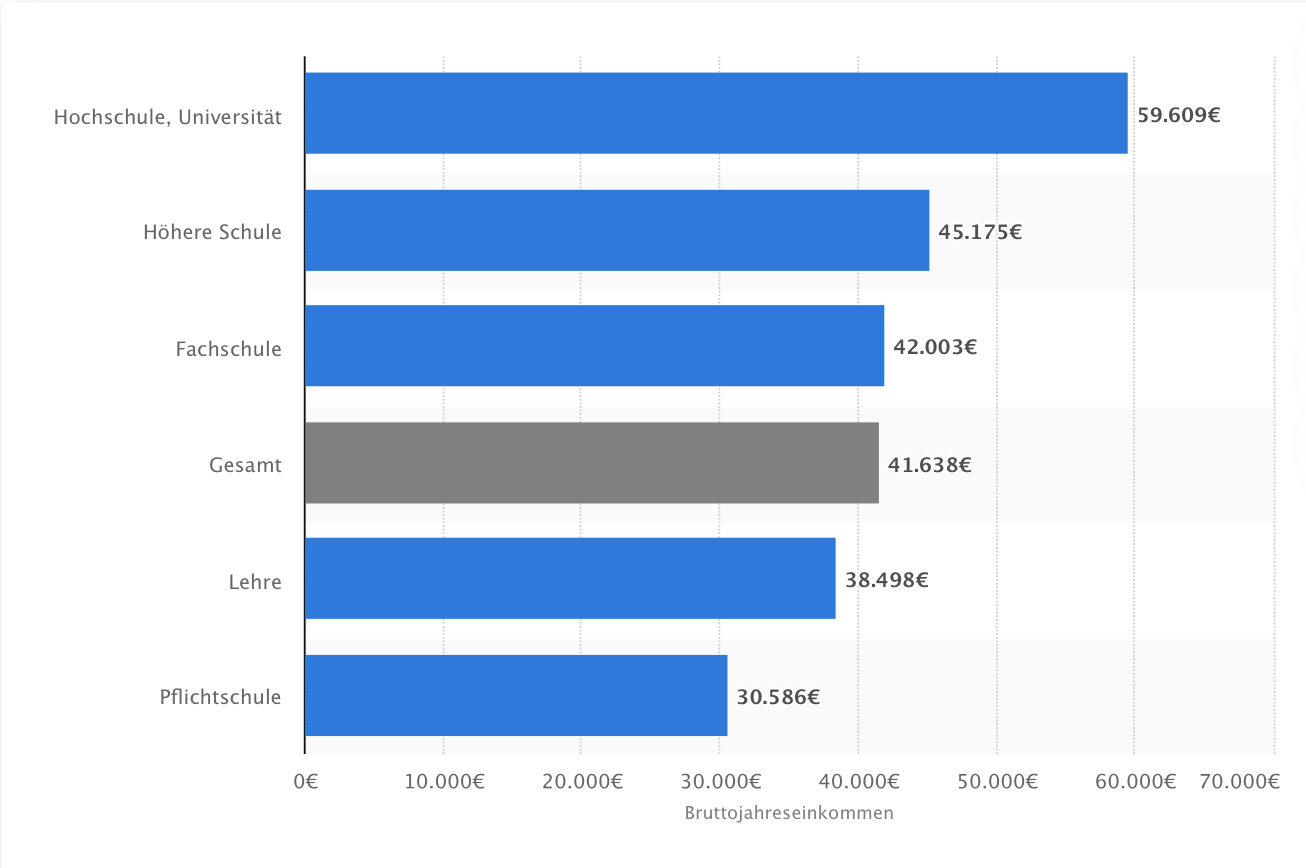
\includegraphics[width=0.7\textwidth]{figures/earnings_austria_2017}
\end{center}
{\tiny Source: Statistik Austria, Statista 2022}

%================================================================
\foilhead{Purpose of this course}

\bi 
\x Understand program evaluation as a \textit{consumer}
\bi
\xx Synthesize and understand evaluation results
\xx Evaluate the quality of policy evaluations or choose between evaluation proposals
\xx Make evidence-based decisions
\ei
\pause
\x Provide skills to design and implement program evaluations

\bi 
\xx Many economists work on evaluations, not only in academia
\ei

\ei

%================================================================
\renewcommand{\sectiontitle}{5.1 Introduction and basic concepts}
%================================================================

%================================================================
\foilhead{Why do we evaluate programs?}

\bi
\x {\textit {Policy}} and {\textit {program}} will be used as synonyms
\x Lots of money is spent every year to try to change things
\bi
\xx government-provided job training programs
\xx sugar-tax to reduce obesity
\xx subsidies to increase R\&D investment in firms
\xx incentive schemes to increase worker productivity
\ei
\x We want to know:
\bi
\xx What difference have these programs made?
\xx What outcomes have been affected? By how much and for whom?
\ei
\ei

%================================================================
\foilhead{Broader agenda: Evidence-based policy making}
\bi 
\x Policy decisions informed by rigorously established evidence
\bi 
\xx In reality often: \textit{Policy-based evidence making}
\ei
\x Based on idea of evidence-based medicine
\x Goal: Inform allocation of resources, guide policy decisions, enhance accountability
\x Build general knowledge about the effectiveness of policies
\ei

%================================================================
\foilhead{Which policies should we evaluate}
\begin{small}

\bi 
\x Evaluations are costly, especially data collection
\x What are the stakes of this policy?
\bi 
\xx Budget
\xx Size of target population
\xx {\textit{Potential}} effect sizes
\ei
\x Evaluate if the policy is
\bi 
\xx Innovative: new and promising
\xx Replicable: can be scaled up or be applied in a different setting
\xx Strategically relevant: flagship initiative, requires substantial resources, 
potentially covers a large number of people, could have large (side) effects or generate substantial savings
\xx Untested: Little is known about the effectiveness of this type of policy
\xx Influential: Results will be used to inform key policy decisions
\ei
\ei
\end{small}

%================================================================
\foilhead{Common errors}

\begin{small}
\bi 
	\x People without knowledge in program evaluation tend to confuse 
	\bi 
		\xx monitoring and evaluation
		\xx correlation and impacts
	\ei
	\x Examples
	\bi 
		\xx The program was successful: 72\% of participants find a job after job training
		\xx I feel better today, because I took Globuli yesterday
		\xx She has a high income, because she studied economics
		\xx Aztecs: without human sacrifices of children, rain would not come and crops would not flourish
	\ei
	\x This can be extremely misleading
\ei
\end{small}

%================================================================
\foilhead{Simpson's (1951) paradox}

\bi 
\x Event C increases probability of E in population, whereas it decreases probability of E in all sub-populations
\x Example: Taking a particular pill is helpful for the population but harmful for men and women
\ei
\pause
\begin{tabular}{lcccc}\hline 
Combined&recovery (E)&not E & sum & recovery rate \\\hline 
Drug (C)&20&20&40&50\%\\
No drug (not C)&16&24&40&40\%\\\hline 
  \end{tabular}

%================================================================
\foilhead{Simpson's (1951) paradox}

\begin{tabular}{lcccc}\hline 
Men&recovery (E)&not E & sum & recovery rate \\\hline 
Drug (C)&18&12&30&60\%\\
No drug (not C)&7&3&10&70\%\\\hline 
  \end{tabular}

\begin{tabular}{lcccc}\hline 
Women&recovery (E)&not E & sum & recovery rate \\\hline 
Drug (C)&2&8&10&20\%\\
No drug (not C)&9&21&30&30\%\\\hline 
  \end{tabular}
\vspace{1cm}

\textbf{What is going on?}


%================================================================
\foilhead{Simpson's (1951) paradox}

\bi 
	\x Drug appears to be beneficial in for the population because
	\bi 
		\xx men recover more often than women with and without taking the drug \&
		\xx men are more likely than women to take the drug
	\ei
	\x In other words, sex is a confounder and needs to be controlled for the obtain valid causal conclusions
	\x Other example: UC-Berkeley investigation for sex-bias in graduate admissions (1975)
\ei


%================================================================
\foilhead{What is impact evaluation?}

\bi
\x \textbf{Monitoring} tracks what is happening with a program, looks at the program implementation
\bi
\xx Is the money indeed spent the way it was supposed to be?
\ei
\x \textbf{Impact evaluations} seek to answer a cause-and-effect question
\bi
\xx Which changes are directly attributably to a program?
\xx What is the effect of obtaining a university degree on earnings?
\ei
\ei

%================================================================
\foilhead{What is impact evaluation?}

The central idea of any impact evaluation is to estimate the so-called \textbf{counterfactual}.

What the outcome would have been for program participants if they had not participated in
the program.

Why is this difficult? For any given person/unit we observe the outcome only in the treated or untreated state, never in both!

%================================================================
\foilhead{Prospective versus retrospective evaluation}

\bi 
\x {\textbf{Prospective evaluation}}
\bi 
\xx Set up at the same time as policy
\xx Built into policy implementation / roll-out
\ei
\x {\textbf{Retrospective evaluation}}
\bi 
\xx Policy evaluation after implementation
\ei
\x PE more likely to produce credible evaluation results
\bi 
\xx (Baseline) data collection on treated and controls
\xx Creates focus on policy objectives
\xx Easier to construct credible counterfactual
\ei
\ei

%================================================================
\foilhead{Efficacy studies and effectiveness studies}

\bi 
\x {\textbf{Efficacy studies}}
\bi 
\xx Carried out in a specific setting under closely controlled conditions
\xx Small-scale pilot / proof of concept
\ei
\x {\textbf{Effectiveness studies}}
\bi 
\xx Interventions that take place in normal circumstances, using regular implementation channels
\xx Aim to produce findings that can be generalized to a large population
\ei
\ei
%================================================================
\foilhead{Internal versus external validity}

\bi 
\x {\textbf{Internal validity}}
\bi 
\xx Evaluation identifies causal effect of program in a given setting
\xx Varying degrees of credibility (RCT: Gold Standard)
\ei
\x {\textbf{External validity}} 
\bi 
\xx Generalizability of causal effect to other situation
\xx Informative for larger or different population, different time
\ei
\pause
\x Economists argue about their relative importance (Deaton 2010)
\bi 
\xx High degree of internal validity often easier in settings with low external validity (e.g. lab experiments with college students)
\ei
\ei

%================================================================
\foilhead{Cost-benefit and cost-effectiveness analysis}
\bi
\x \textbf{Cost-benefit analysis}
\bi
\xx Estimates the total expected benefits of a program, compared to its total
expected costs. 
\xx Seeks to quantify all of the costs and benefits of a program
in monetary terms and assesses whether benefits outweigh costs.
\ei
\x \textbf{Cost-effectiveness analysis}
\bi
\xx Compares the relative cost of two or more programs
or program alternatives in reaching a common outcome
\ei
\ei
Impact evaluation estimates the benefit side, and cost analysis provides
the cost information! We focus on \textbf{impact evaluation}.

%================================================================
%\foilhead{Ethical considerations}

%DECIDE WHETHER HERE OR LATER (p. 20 or 21 in the book)

%================================================================
\foilhead{Preparing for an evaluation}

\bi
\x Specify the evaluation question
\x Construct a theory of change
\x Develop a results chain
\x Select indicators to assess performance
\ei

%================================================================
\foilhead{Evaluation question}

\bi 
\x First step: Formulate a clear study question
\bi 
\xx What is the impact of the policy on an outcome of interest?
\xx Which changes are directly attributable to a program?
\ei
\x Needs to be framed as a \textbf{well-defined, testable hypothesis}
\ei

%================================================================
\foilhead{Are these good evaluation questions?}

\bi
\x What is the effect of studying economics on later earnings?
\x What is the effect of being a woman on the likelihood of becoming a politician?
\x What is the effect of reducing the speed limit on highways from 130 to 100 km/h on the number of traffic deaths?
\ei

%================================================================
\foilhead{Theory of change}

\bi 
\x Describe the causal pathway (sequence of events from policy to final outcomes)
\x Formulate necessary assumptions and enabling conditions
\x Include all stakeholders
\x Consult existing literature
\ei
Can be based on formal model or simply as a results chain.



%================================================================
\foilhead{Results chain}

\begin{center}
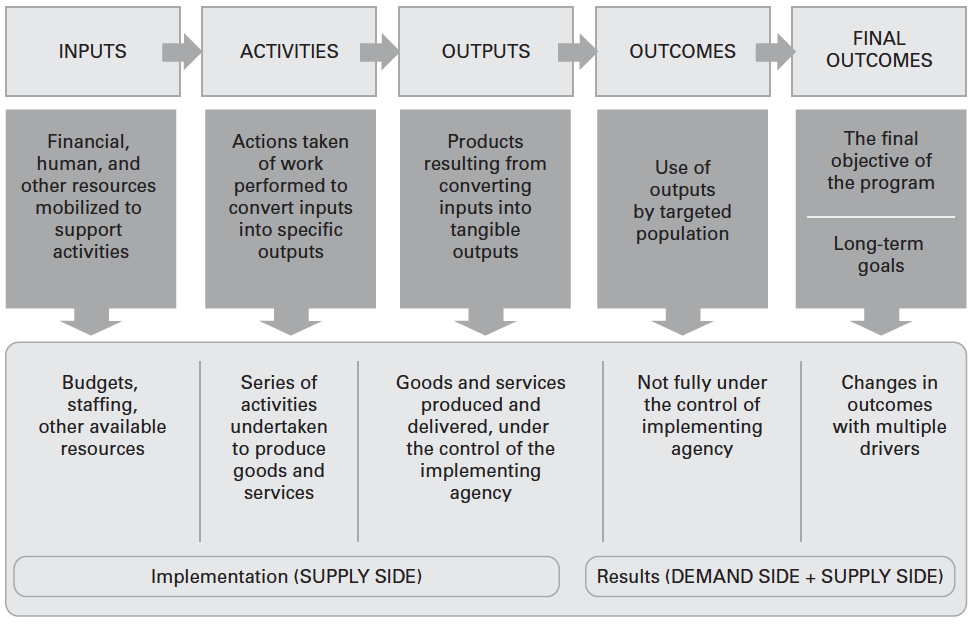
\includegraphics[width=0.9\textwidth]{figures/results_chain}
\end{center}

\begin{comment}
\begin{small}
\bi 
\x Causal logic about the sequence of inputs, activities, and outputs that affect final outcomes
\bi 
\xx {\textbf{Inputs}}: Resources at the disposal of the project, including staff and
budget.
\xx {\textbf{Activities}}: Actions taken or work performed to convert inputs into
outputs.
\xx {\textbf{Outputs}}: Tangible goods and services produced; under the control of the implementing agency.
\xx {\textbf{Outcomes}}: Use of outputs by target population; usually achieved in the short to medium
term; not directly under the control of the implementing agency.
\xx {\textbf{Final outcomes}}: Final objective of the program; influenced by multiple; achieved over a longer period of time.
\ei
\ei
\end{small}
\end{comment}

%================================================================
\foilhead{Results chain - example}

\begin{small}

\bi 
\x Government agency provides trainings about settlement to immigrants
\bi 
\xx {\textbf{Inputs}}: Staff from government agency, trainers, facilities, government budget, contact information of immigrants
\xx {\textbf{Activities}}: Design curriculum of training, select and prepare trainers, design, prepare, and distribute written material
\xx {\textbf{Outputs}}: Number of immigrants trained, number of written materials provided
\xx {\textbf{Outcomes}}: Immigrants behave differently (smarter) based on information provided
\xx {\textbf{Final outcomes}}: Immigrants are (economically) more successful, higher well-being, less welfare spending for immigrants, reduced social tensions
\ei
\ei
\end{small}


%================================================================
\foilhead{Performance indicators (Outcomes)}
{\small
\bi 
\vspace{-1em}
\x Ideally use indicators along the whole results chain
\bi 
\xx Not only final outcomes
\xx Understand mechanisms
\xx Especially important if evaluation finds no effect on final outcome
\ei
\x Selection of indicators should involve stakeholders
\x SMART indicators 
\bi 

\xx Specific: translates required information into operational measure
\xx Measurable: information can be measured and obtained
\xx Attributable: indicator is linked to the policy's efforts
\xx Realistic: information can be obtained timely, with reasonable frequency, at reasonable cost
\xx Targeted: to the objective population 
\ei
\ei
}

\end{document}
